\documentclass[tikz,border=6pt]{standalone}
\usepackage{ctex}
\usepackage{amsmath}
\usetikzlibrary{calc, arrows.meta}

\begin{document}
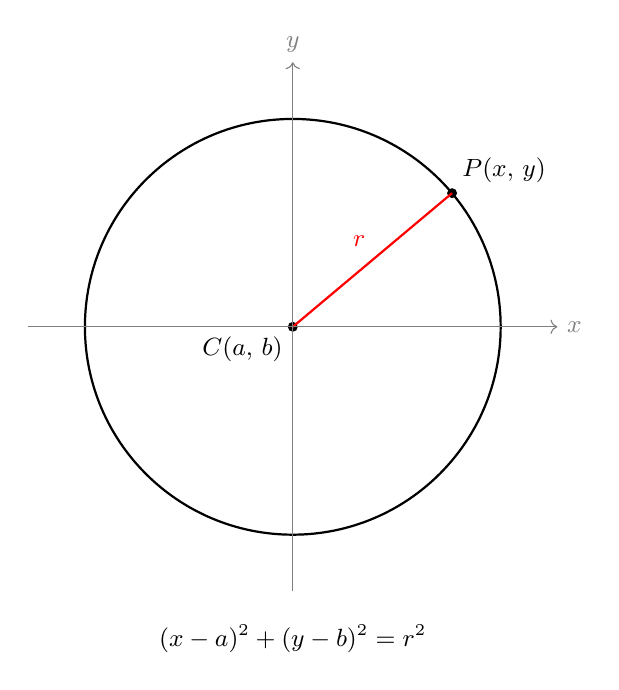
\begin{tikzpicture}[scale=1.2, thick]

% 圆：圆心 C(a,b)，半径 r
\coordinate (C) at (0, 0);
\coordinate (P) at (2.5, 1.5);  % 圆上动点，满足 |CP|=r

% 计算半径（使 P 真正在圆上）
% 让 r = 2.0，P 在圆上：取 P = (2*cos(30.96°), 2*sin(30.96°)) ≈ (1.714, 1.029)
% 重新设定：r=2.2，P = (2.2*cos(40°), 2.2*sin(40°))
\coordinate (Center) at (0, 0);

% 画圆（半径 2.2）
\draw[black, thick] (Center) circle [radius=2.2];

% 标圆心
\fill[black] (Center) circle [radius=1.5pt];
\node[below left, font=\small] at (Center) {$C(a,\,b)$};

% 动点 P（在圆上）
\coordinate (Pt) at ({2.2*cos(40)}, {2.2*sin(40)});
\fill[black] (Pt) circle [radius=1.5pt];
\node[above right, font=\small] at (Pt) {$P(x,\,y)$};

% 半径 CP，用红色标注
\draw[red, thick] (Center) -- (Pt);

% 标 |CP| = r，放在线段中点上方
\node[red, font=\small, above left] at ($(Center)!0.52!(Pt)$) {$r$};

% 虚线：从圆心到 x 轴作垂线（辅助理解圆心位置）
\draw[gray, dashed, thin] (Center) -- (0, -2.5);
\draw[gray, dashed, thin] (Center) -- (-2.5, 0);

% 坐标轴
\draw[->, thin, gray] (-2.8, 0) -- (2.8, 0) node[right, font=\small] {$x$};
\draw[->, thin, gray] (0, -2.8) -- (0, 2.8) node[above, font=\small] {$y$};

% 圆心坐标辅助点
\fill[gray] (0, 0) circle [radius=0pt]; % 原点
\node[below right, font=\footnotesize, gray] at (0, 0) {};

% 标注圆的方程
\node[font=\small, align=center] at (0, -3.3)
  {$(x-a)^2+(y-b)^2=r^2$};

\end{tikzpicture}
\end{document}
